\documentclass[a4paper, 12pt]{article}
\usepackage[a4paper,top=1.5cm, bottom=1.5cm, left=1cm, right=1cm]{geometry}

% Работа с русским языком
\usepackage[utf8]{inputenc}
\usepackage{mathtext}                % русские буквы в формулах
\usepackage[english, russian]{babel} % локализация и переносы

\usepackage{graphicx}   % Вставка изображений
\usepackage{float}      % "Плавающие" изображения3
\usepackage{wrapfig}    % Обтекание фигур (таблиц, картинок и прочего)
\usepackage{subfig}
\graphicspath{ {./images/} }

\usepackage{tabularx}
\usepackage{multirow}
\usepackage{booktabs}
\usepackage{amsmath}
\usepackage{amsfonts}
\usepackage{indentfirst}
\usepackage{longtable}
\graphicspath{{pictures/}}
\usepackage{natbib}
\usepackage{bm}

\newcommand{\figref}[1]{(См. рис. \ref{#1})}
\newcommand{\secref}[1]{(См. раздел. \ref{#1})}

\newcommand{\atm}[1][\;]{#1 атм.}
\newcommand{\mmhg}[1][\;]{#1 мм рт.ст.}
\newcommand{\Bk}[1][\;]{#1 Бк}
\newcommand{\MeV}[1][\;]{#1 МэВ}
\newcommand{\keV}[1][\;]{#1 кэВ}
\newcommand{\eV}[1][\;]{#1 эВ}
\newcommand{\msec}[1][\;]{#1 мс}
\renewcommand{\sec}[1][\;]{#1 с}
\renewcommand{\min}[1][\;]{#1 м}
\newcommand{\hour}[1][\;]{#1 ч}
\renewcommand{\day}[1][\;]{#1 д}
\renewcommand{\year}[1][\;]{#1 л}

\newcommand{\stable}[1][\;]{#1 (ст.)}

\newcommand{\elem}[3]{{}^{#2}_{#3}\text{#1}}
\newcommand{\Ra}{\elem{Ra}{226}{88}}
\newcommand{\Pu}{\elem{Pu}{239}{94}}
\newcommand{\Po}{\elem{Po}{210}{84}}
\newcommand{\Ua}{\elem{U}{238}{92}}
\newcommand{\Ub}{\elem{U}{234}{92}}
\newcommand{\Th}{\elem{Th}{230}{90}}
\newcommand{\Am}{\elem{Am}{241}{95}}


%%% Колонтитулы
\usepackage{titleps}
\newpagestyle{main}{
	\setheadrule{0.4pt}
	\sethead{Отчёт о выполнении лабораторной работы 5.2}{}{}
	\setfootrule{0.4pt}                       
	\setfoot{ФРКТ МФТИ, 2024}{}{\thepage} 
}
\pagestyle{main}  

\begin{document}
    \begin{titlepage}
	\begin{center}
            {\large МОСКОВСКИЙ ФИЗИКО-ТЕХНИЧЕСКИЙ ИНСТИТУТ (НАЦИОНАЛЬНЫЙ ИССЛЕДОВАТЕЛЬСКИЙ УНИВЕРСИТЕТ)}
	\end{center}
 
	\begin{center}
		{\large Физтех-школа радиотехники и компьютерных технологий}
	\end{center}
	
	\vspace{8cm}
	{\LARGE
		\begin{center}
                {\bf Отчёт о выполнении лабораторной работы 5.2}\\
                Спектрометрия $\alpha$-излучения с помощью полупроводникового детектора
		\end{center}
	}
	\vspace{4cm}
	\begin{flushright}
		{\Large Авторы: \\ 
        Тихонов Дмитрий Романович, \\ студент группы Б01-206а \\
        Павловский Кирилл Михайлович, \\ студент группы Б01-206а}
	\end{flushright}
	\vspace{4cm}
	\begin{center}
		\Large Долгопрудный, 2024
	\end{center}
    \end{titlepage}


    \section{Введение}

    \noindent \textbf{Цель работы:} измерить спектры $\alpha$-излучения ядер $\Ra$, $\Po$, $\Pu$, $\Ua$ и смеси ($\Th$ и $\Am$) с помощью полупроводникового детектора; исследовать последовательные $\alpha$-распады указанных ядер; проверить закон Гейгера-Нэттола для ядер $\Ra$ на основе табличных значений. \\
	

    \noindent \textbf{В работе используются:} форвакуумный насос Value VE-215N, $\alpha$-спектрометр Амплитуда НТЦ Мультирад-АС, персональный ЭВМ со встроенной платой АЦП, образцы с источниками $\Ra$, $\Po$, $\Pu$, $\Ua$ и смеси ($\Th$ и $\Am$).
    
    \section{Теоретические сведения}
    
    \textit{Альфа-распадом} называется самопроизвольный процесс испускания ядрами альфа-частиц:
    $$
    \elem{X}{A}{Z} \rightarrow \elem{$X'$}{A-4}{Z-2} + \elem{He}{4}{2}
    $$

    Периодом полураспада $T_{1/2}$ называется время, в течение которого количество радиоактивных атомов убывает в 2 раза. Если $N_0$ -- начальное количество радиоактивных атомов, то количество атомов $N(t)$ в последующие моменты времени определяется \textit{законом радиоактивного распада}:
    $$
    N = N_0  \left(\frac{1}{2}\right)^{t / T_{1/2}}
    $$

    Для $\alpha$-распада период полураспада $T_{1/2}$ связан с энергией вылетающий $\alpha$-частиц $E_i$ законом Гейгера-Нэттола:
    \begin{equation}
        \ln T_{1/2} = \frac{a}{\sqrt{E_i}} + b
        \label{eq:geiger_nuttall_law}
    \end{equation}
	
    \textit{Спектром} радиоактивного излучения называется энергетическое распределение исследуемого излучения. В случае $\alpha$-распада спектром будет график зависимости количества зарегистрированных $\alpha$-частиц от их энергии. Прибор, который измеряет спектр радиоактивного излучения называется \textit{спектрометром}. Важной характеристикой спектрометра является его \textit{разрешающая способность} $R$, то есть возможность различить излучение с близкими энергиями. Разрешающая способность прибора определяется разрешающей способностью детектирующего излучение датчика и шумами в электронной схеме.
	
    \begin{figure}[H]
        \centering
        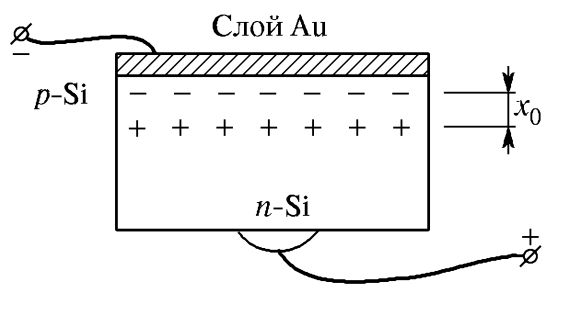
\includegraphics[width=0.45\textwidth]{images/detector.png}
        \caption{Схема полупроводникового детектора.}
        \label{img:detector}
    \end{figure}

    Рассмотрим принцип работы полупроводникового детектора (рис. \ref{img:detector}). Детектор представляет собой обычно кремниевую пластинку из полупроводников $n$- и $p$-типа. В $n$-области находятся свободные электроны, в $p$-области находятся свободные дырки. Когда к пластинке прикладывается постоянное напряжение, как показано на рисунке, то свободные заряды покидают пластинку, в результате чего проводимость детектора уменьшается, при этом образуется обеднённая область шириной $x_0$. Альфа-частица энергией $E_i$ пролетает через обеднённую область детектора и ионизует атомы полупроводника, переводя электроны из валентной зоны в свободную. В результате ионизации образуется пара электрон-дырка и возникает ток под действием приложенного к детектору напряжения. Этот ток усиливается зарядочувствительным усилителем, напряжение на котором пропорционально заряду, протекающему через усилитель. Напряжение на усилителе измеряется АЦП. Ток через усилитель пропорционален числу образованных пар электрон-дырка в детекторе. На образование одной такой пары в среднем расходуется энергия $E_{ср} = 3.6 \eV$. Предполагая, что $\alpha$-частица расходует всю свою энергию $E_i$ на ионизацию атомов в обеднённом слое, можно оценить среднее количество образовавшихся пар электрон-дырка $N$:
    $$
    N_i = \frac{E_i}{E_{ср}}
    $$

    Предполагается, что ионизация атомов происходит независимо друг от друга с фиксированной интенсивностью, тогда количество ионизованных атомов подчиняется распределению Пуассона. Так как $N_i$ велико ($E_i \sim 1 \MeV$, $N_i \sim 10^5$), то распределение Пуассона приближается к распределению Гаусса с средним значением $N_i$ и среднеквадратичным отклонением $\sigma = \sqrt{N_i}$. \textit{Разрешающая способность детектора} определяется как отношение среднеквадратичного отклонения к среднему значению:
    $$
    R_{фл} = \frac{\sqrt{N_i}}{N_i} = \frac{1}{\sqrt{N_i}}
    $$
	
    Пусть в измеренной спектрограмме средняя энергия $\alpha$-частиц составляет $E_i$, полуширина пика на половине высоты $\Delta E_i$, тогда \textit{энергетическая разрешающая способность} спектрометра равна:
    $$
    R = \frac{\Delta E_i}{E_i}
    $$

    Разрешающая способность спектрометра зависит от разрешающей способности детектора и от уровня шума в электронной схеме.

    \newpage
    
    \section{Методика измерений и экспериментальная установка}

    \subsection{Описание экспериментальной установки}	
    
    Схема экспериментальной установки приведена на рисунке \ref{img:exp_scheme}:
        
    \begin{figure}[H]
        \centering
        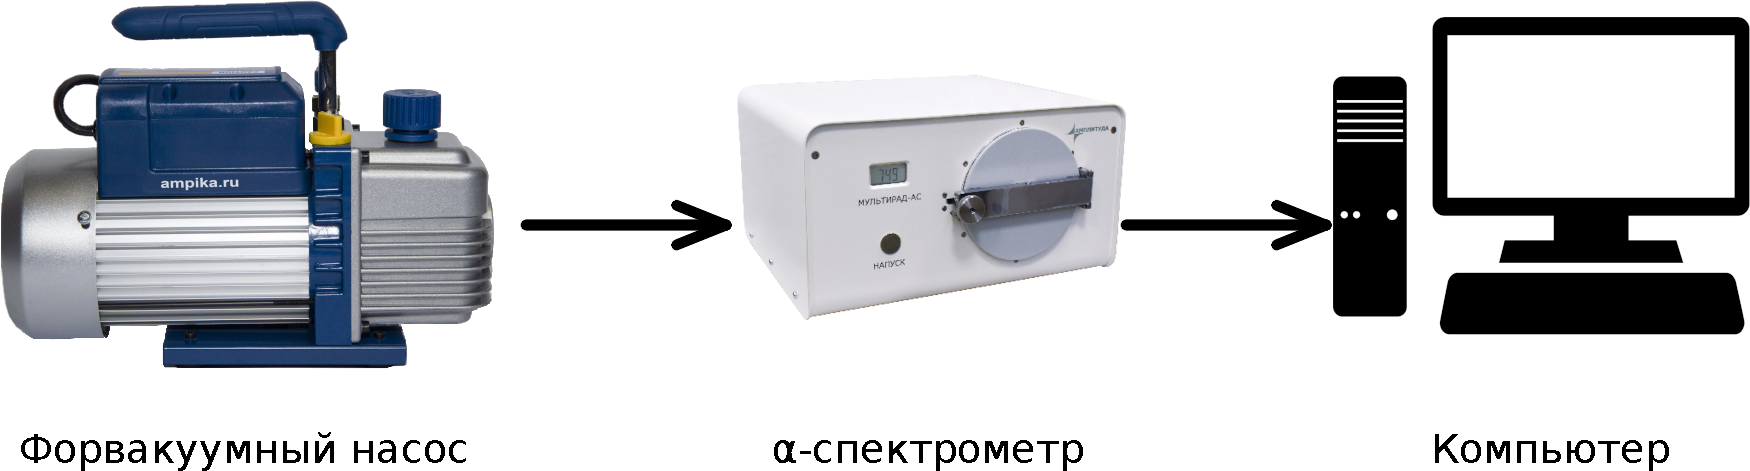
\includegraphics[width=1\textwidth]{images/exp_scheme.png}
        \caption{Схема экспериментальной установки.}
        \label{img:exp_scheme}
    \end{figure}

    Форвакуумный насос соединён с корпусом $\alpha$-спектрометра вакуумным шлангом для откачки измерительной камеры до давлений $0.4 \div 20 \mmhg$. В камеру $\alpha$-спектрометра на специальный столик помещается радиоактивный препарат. Над столиком находится полупроводниковый детектор частиц, который регистрирует $\alpha$-частицы в диапазоне энергий $4.0 \div 9.5 \MeV$. Сигнал с детектора усиливается и подаётся на 12-битный АЦП. То есть спектрометр имеет 4096 каналов измерения энергий $\alpha$-частиц. Результаты измерений передаются на компьютер, который проводит первичную обработку данных -- строит спектр радиоактивного распада. На подложку стола подаётся отрицательный относительно корпуса потенциал, чтобы ядра отдачи с импульсом направленным к детектору не попадали на него и не загрязняли его.

    \subsection{Оборудование и приборы}
		
    \begin{itemize}
        \item Форвакуумный насос Value VE-215N. Остаточное давление: $0.00002 \; \atm = 0.0152 \;\mmhg$.
		
        \item Альфа-спектрометр Амплитуда НТЦ Мультирад-АС. Диапазон энергии регистрируемого излучения $4.0 \div 9.5 \MeV$. Диапазон измерения активности $1 \cdot 10^2 \div 5 \cdot 10^5 \Bk$. Пределы допускаемой основной относительной погрешности измерений активности в исследуемых образцах $\varepsilon = 10 \%$. Максимальное значение входной нагрузки статистически распределённых импульсов не менее $10^4 \; \frac{имп}{с}$. Диапазон поддерживаемого в камере давления $0.4 \div 20.0 \mmhg$. Уровень собственного фона не более $100 \frac{имп}{сутки}$.
    \end{itemize}
	
    \subsection{Методика эксперимента}
	
    Так как зависимость энергии $\alpha$-частицы от номера зарегистрировавшего её канала спектрометра не известна, то в начале работы проводится градуировка детектора. Для этого измеряется спектр излучения $\Ra$ в течение примерно 10 минут, каждому пику на графике спектра ставится в соответствие энергия зарегистрированной $\alpha$-частицы. Так как амплитуда сигнала на выходе детектора пропорциональна энергии $\alpha$-частицы, то градуировочная кривая должна быть прямой.
	
    После градуировки детектора измеряются спектры $\Po$, $\Pu$, $\Ua$ и смеси ($\Th$ и $\Am$) в течение примерно 10 минут. По градуировочной зависимости определяются энергии зарегистрированных $\alpha$-частиц, и по справочнику определяются атомы, в результате радиоактивного распада которых образовалась $\alpha$-частица.

    \newpage
	
    \section{Результаты измерений и обработка данных}

    \subsection{Градуировка детектора}
    По известным значениям энергии $\alpha$-частицы при распаде $\Ra$ и его дочерних ядер, определяются коэффициенты $a$ и $b$ градуировочной кривой детектора:
    $$
    E_i = a\cdot N_i + b.
    $$
	
    График градуировочной кривой $E_i(N_i)$ изображен на рисунке \ref{fig:w-channel}. С помощью метода наименьших квадратов были получены следующие градуировочные коэффициенты:
	
    $$ a = (2.97 \pm 0.01) \cdot 10^{-3} \; \frac{ \text{МэВ} }{ \text{кан.} },$$
    $$ b = (-0.10 \pm 0.02) \; \text{МэВ}.$$
	
    \begin{figure}[H]
        \centering
        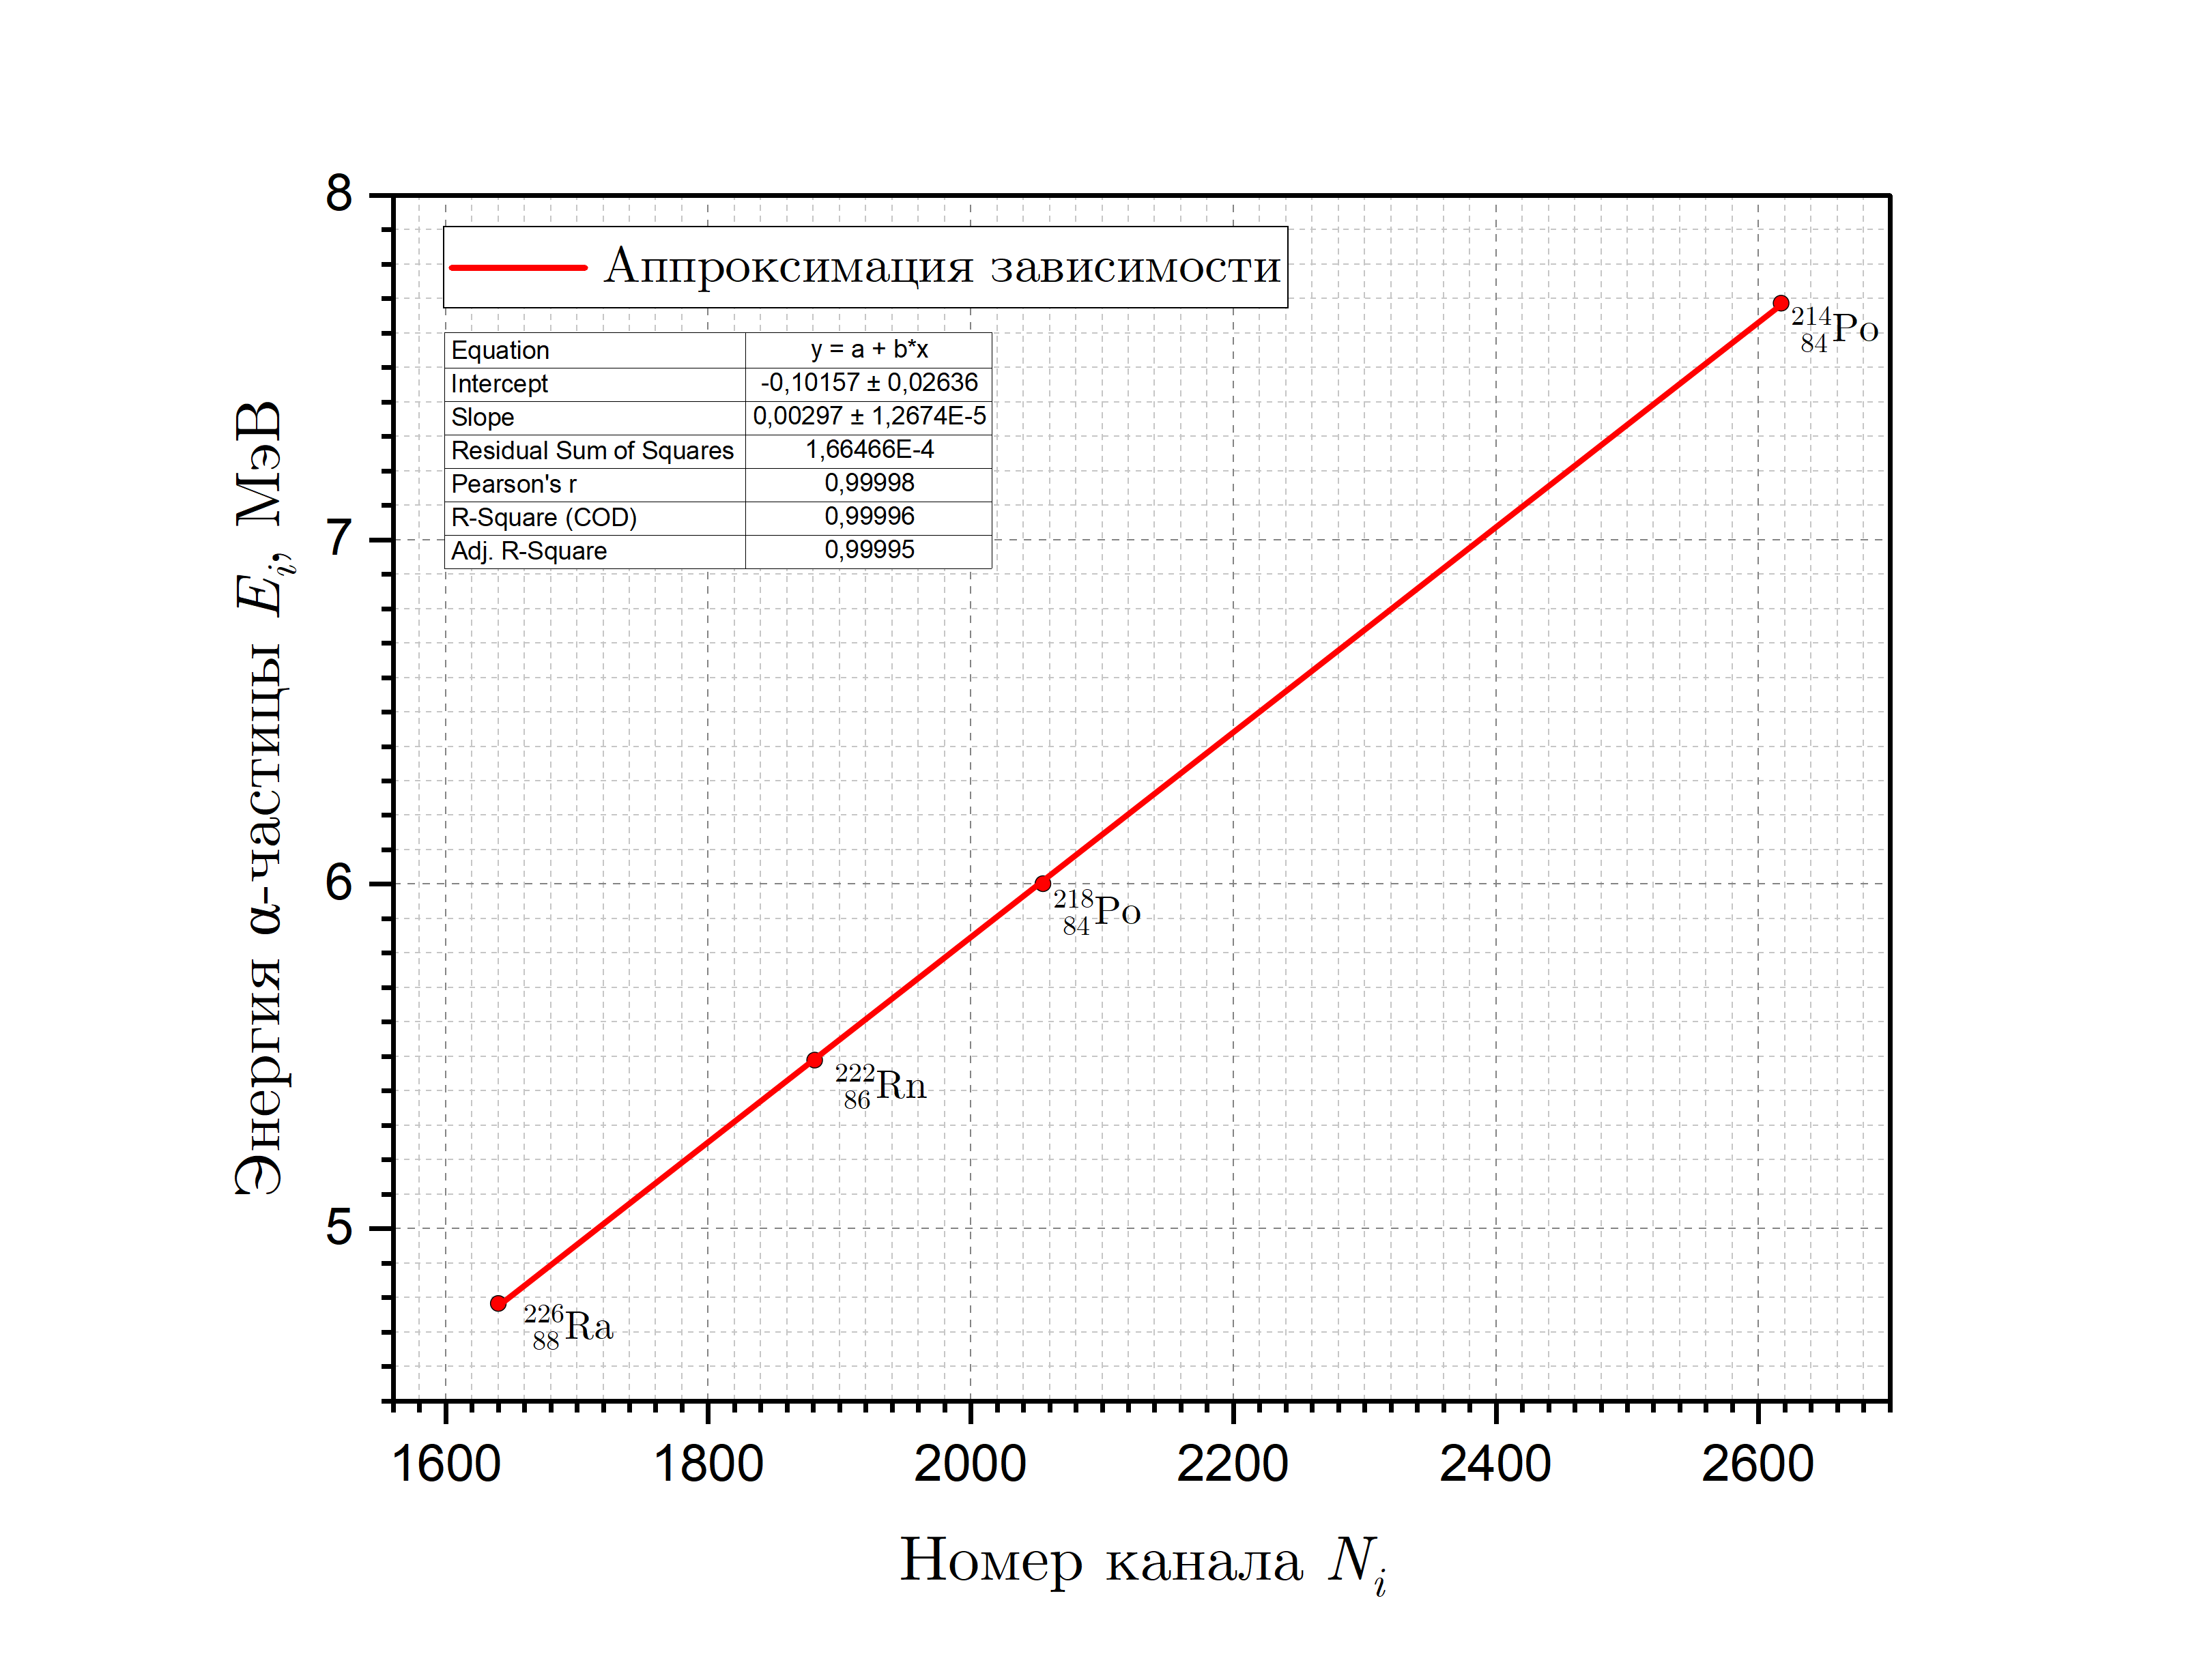
\includegraphics[width = 12 cm]{images/calibration_graph .png}
        \caption{Зависимость энергии $\alpha$-частицы от номера канала $E_i(N_i)$.}
        \label{fig:w-channel}
    \end{figure}
	
    Согласно теории сдвиг по энергии $b$ должен быть равен 0. Систематическая ошибка, вносимая этим сдвигом $\varepsilon \sim 2\%$. Далее в таблицах будет приведена только случайная составляющая ошибок, чтобы иметь представление об их порядке. Полная погрешность оценивается по формуле:
    
    $$\varepsilon_\Sigma = \sqrt{\varepsilon^2 + \varepsilon_{E_i}^2}$$
	
    \subsection{Исследование спектров $\alpha$-распада}
	
    С помощью градуировочной зависимости, определялась энергия альфа-частиц для всех остальных элементов: $\Ra$, $\Am + \Th$, $\Pu$, $\Ua$.
	
    В таблицах для каждой последовательности радиоактивных распадов приведены: $N_i$ -- средний номер канала, зарегистрировавший альфа-частицу с фиксированной энергией, $\Delta N_i$ -- среднеквадратичное отклонение в единицах каналов, $E_i$ -- средняя энергия зарегистрированных альфа-частиц, ширина $\Delta E_i$ -- среднеквадратичное отклонение в энергетических единицах, $\sigma_x$ -- случайная составляющая  ошибки определения величины $x$.
	
    Оценка погрешности проводилась по формуле погрешности косвенных измерений:
    $$ 
    \varepsilon_{R_{f,i}} = \frac{1}{2} \sqrt{\varepsilon_\Sigma^2 + \left(\frac{0.05}{3.60}\right)^2} \sim 1.5 \%
    $$
    
    $$ 
    \varepsilon_{R_i} = \sqrt{\varepsilon_{E_i}^2 + \varepsilon_{\Sigma}^2} \approx  \varepsilon_{\Sigma} \sim 2 \%
    $$
	
    \begin{figure}[H]
        \centering
        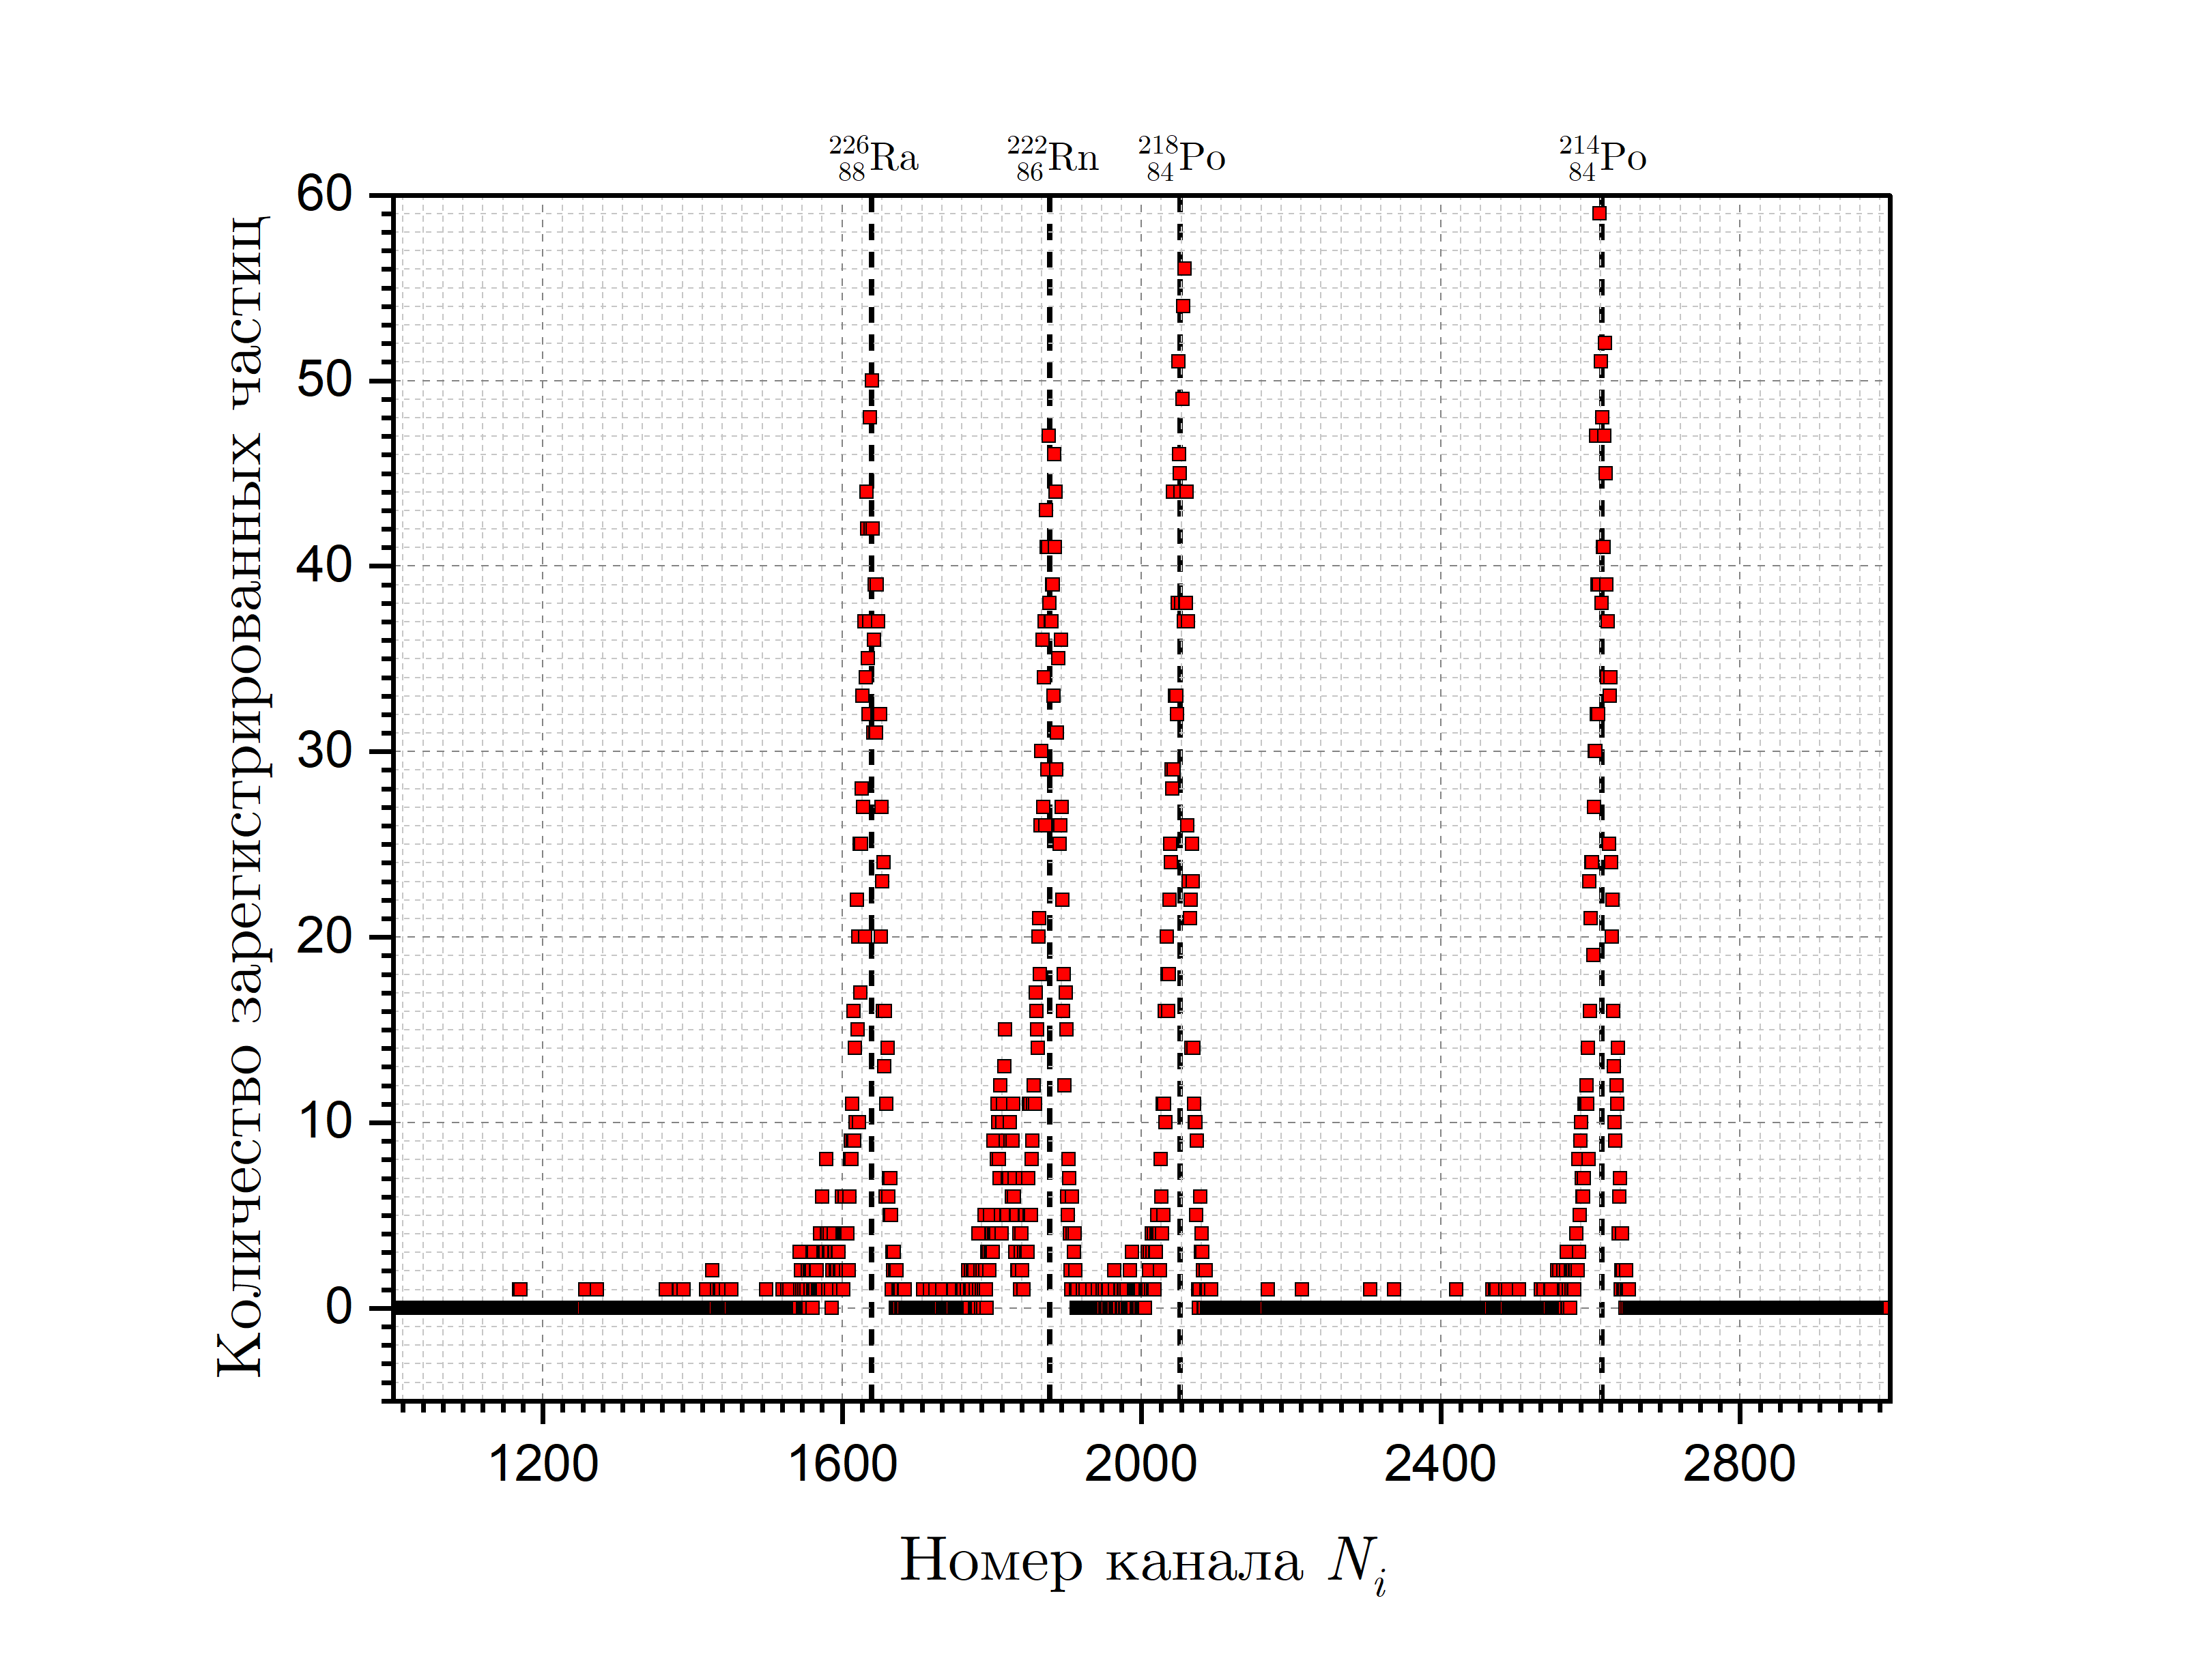
\includegraphics[width = 12 cm]{images/graph_ra.png}
        \caption{Спектр $\Ra$.}
        \label{fig:ra}
    \end{figure}
	
    \begin{table}[H]
        \centering
        \addtolength{\tabcolsep}{-4pt}
        \footnotesize
        \begin{tabular}{cccccc}
            \toprule
            $N_i$ & $dN_i$ & $E_i$, МэВ & $\sigma_{E_i}$, МэВ & $\Delta E_i$, МэВ & $\sigma_{\Delta E_i}$, МэВ \\
            \midrule
            1640.0 & 24.33 & 4.78 & 0.03 & 0.0723 & 0.0003 \\
            1881.0 & 23.97 & 5.49 & 0.03 & 0.0712 & 0.0003 \\
            2055.0 & 21.05 & 6.01 & 0.03 & 0.0626 & 0.0002 \\
            2617.0 & 22.50 & 7.68 & 0.04 & 0.0669 & 0.0002 \\
            \bottomrule
        \end{tabular}
        \caption{Энергии пиков $\Ra$.}
        \label{tab:term}
    \end{table}
	
    \begin{figure}[H]
        \centering
        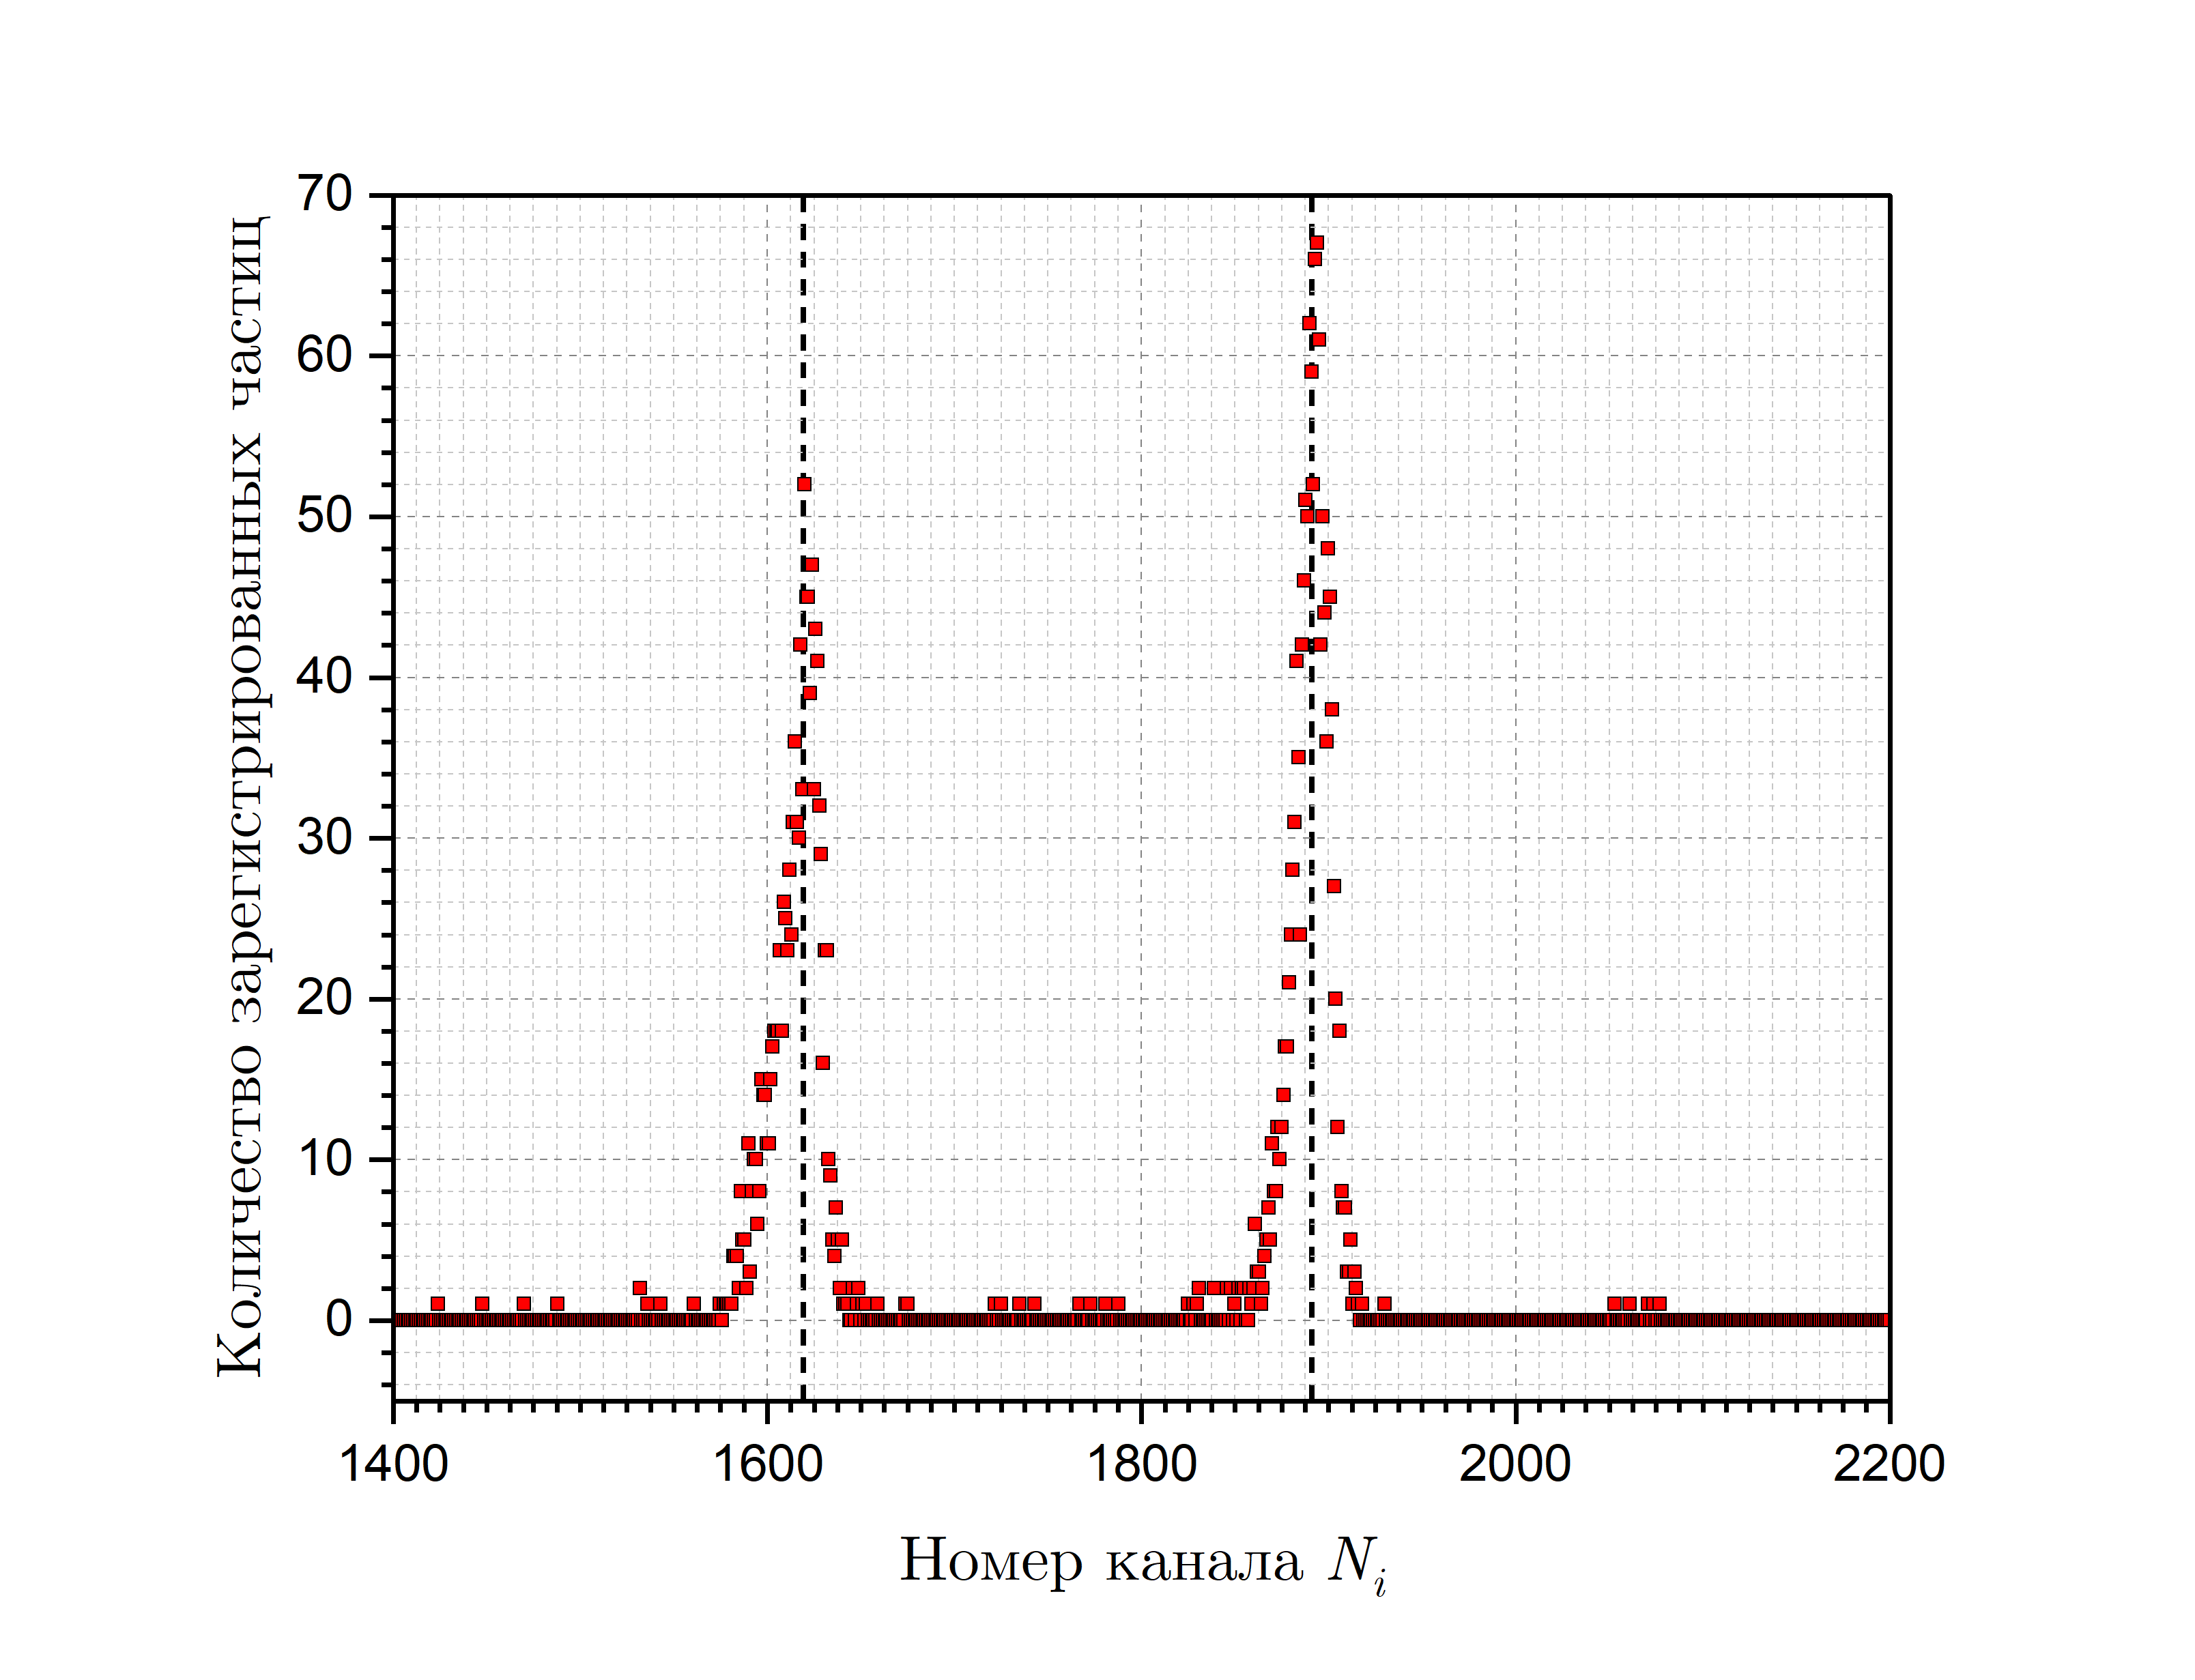
\includegraphics[width = 12 cm]{images/graph_ThAm.png}
        \caption{Спектр $\Am + \Th$.}
        \label{fig:th_am}
    \end{figure}
	
    \begin{table}[H]
        \centering
        \addtolength{\tabcolsep}{-4pt}
        \footnotesize
        \begin{tabular}{ccccccc}
            \toprule
            $N_i$ & $\Delta N_i$ & $E_i$, МэВ & $\varepsilon_{E_i}, \%$ & $\Delta E_i$, МэВ & $R_i \cdot 10^2$ & $R_{f,i} \cdot 10^2$ \\
            \midrule
            1622 & 15.80 & 4.73 & 0.6 & 0.0469 & 0.99 & 0.087 \\
            1894 & 17.12 & 5.53 & 0.6 & 0.0509 & 0.92 & 0.081 \\
            \bottomrule
        \end{tabular}
        \caption{Энергии пиков $\Am + \Th$.}
        \label{tab:th_am}
    \end{table}
	
    \begin{figure}[H]
        \centering
        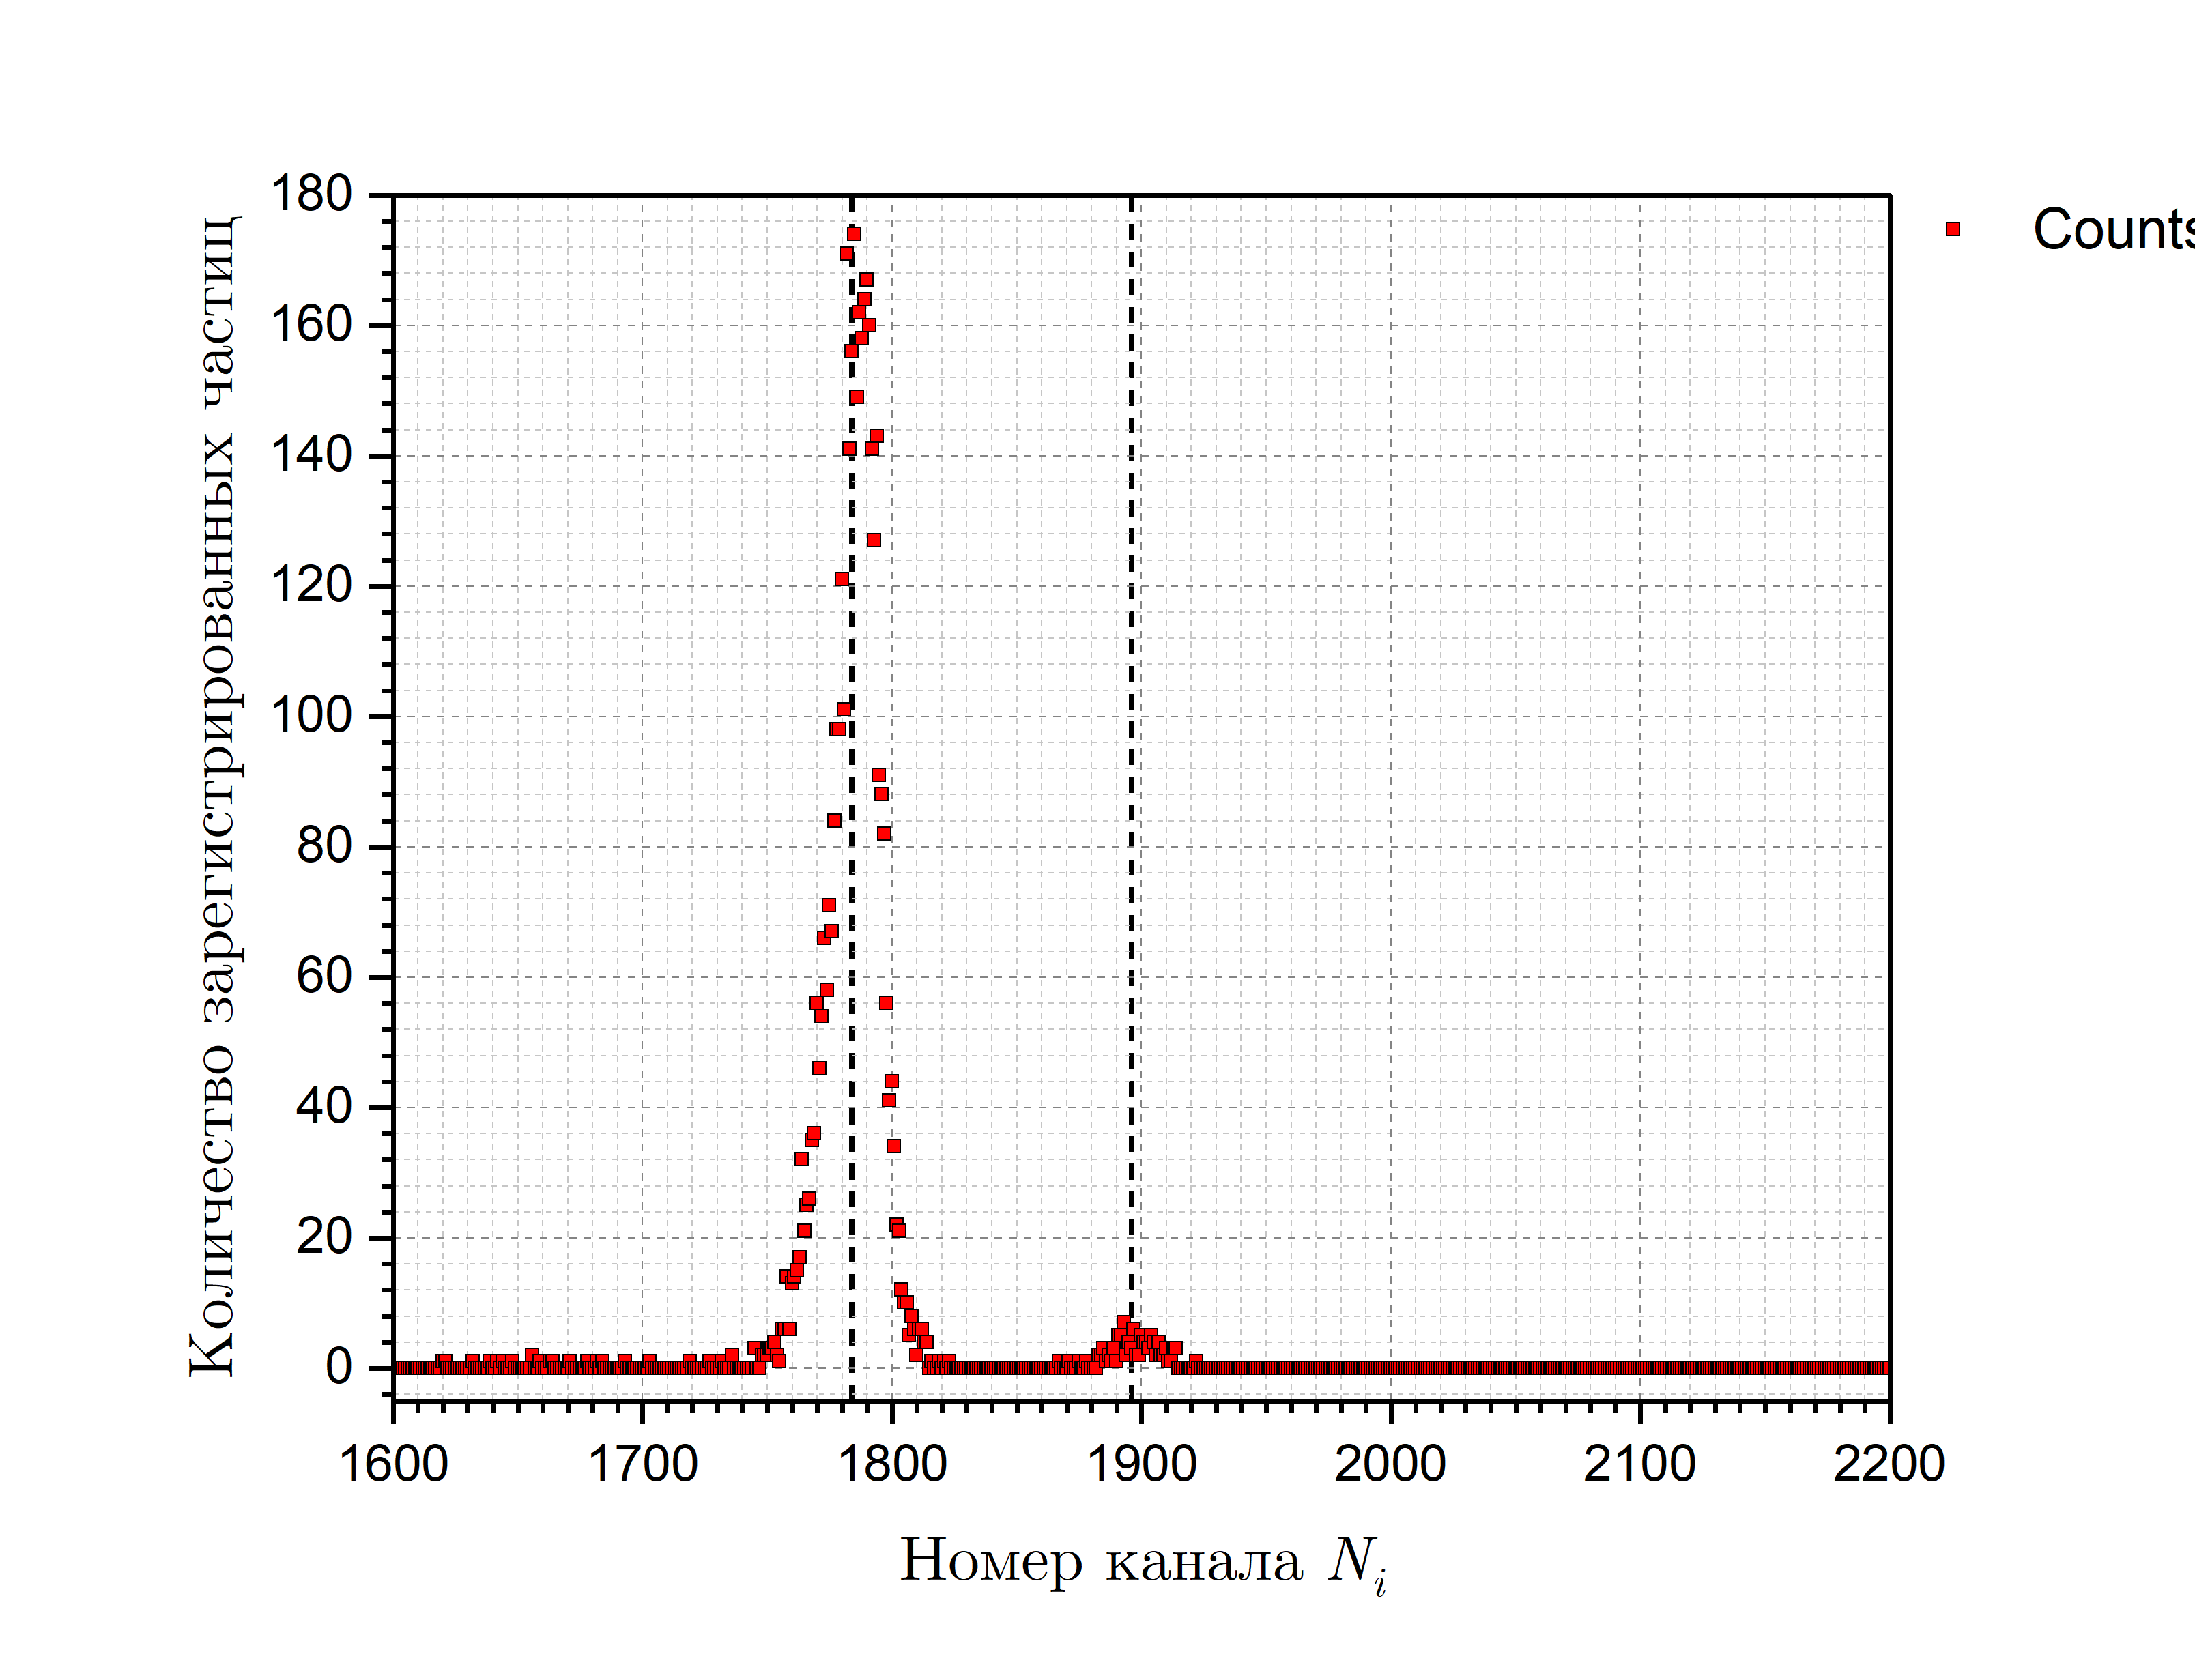
\includegraphics[width = 12 cm]{images/graph_pu.png}
        \caption{Спектр $\Pu$.}
        \label{fig:pu}
    \end{figure}
	
    \begin{table}[H]
        \centering
        \addtolength{\tabcolsep}{-4pt}
        \footnotesize
        \begin{tabular}{ccccccc}
            \toprule
            $N_i$ & $\Delta N_i$ & $E_i$, МэВ & $\varepsilon_{E_i}, \%$ & $\Delta E_i$, МэВ & $R_i \cdot 10^2$ & $R_{f,i} \cdot 10^2$ \\
            \midrule
            1788 & 16.81 & 5.22 & 0.6 & 0.0500 & 0.96 & 0.083 \\
            1894 & 20.90 & 5.53 & 0.6 & 0.0621 & 1.12 & 0.081 \\
            \bottomrule
        \end{tabular}
        \caption{Энергии пиков $\Pu$.}
        \label{tab:pu}
    \end{table}
	
    \begin{figure}[H]
        \centering
        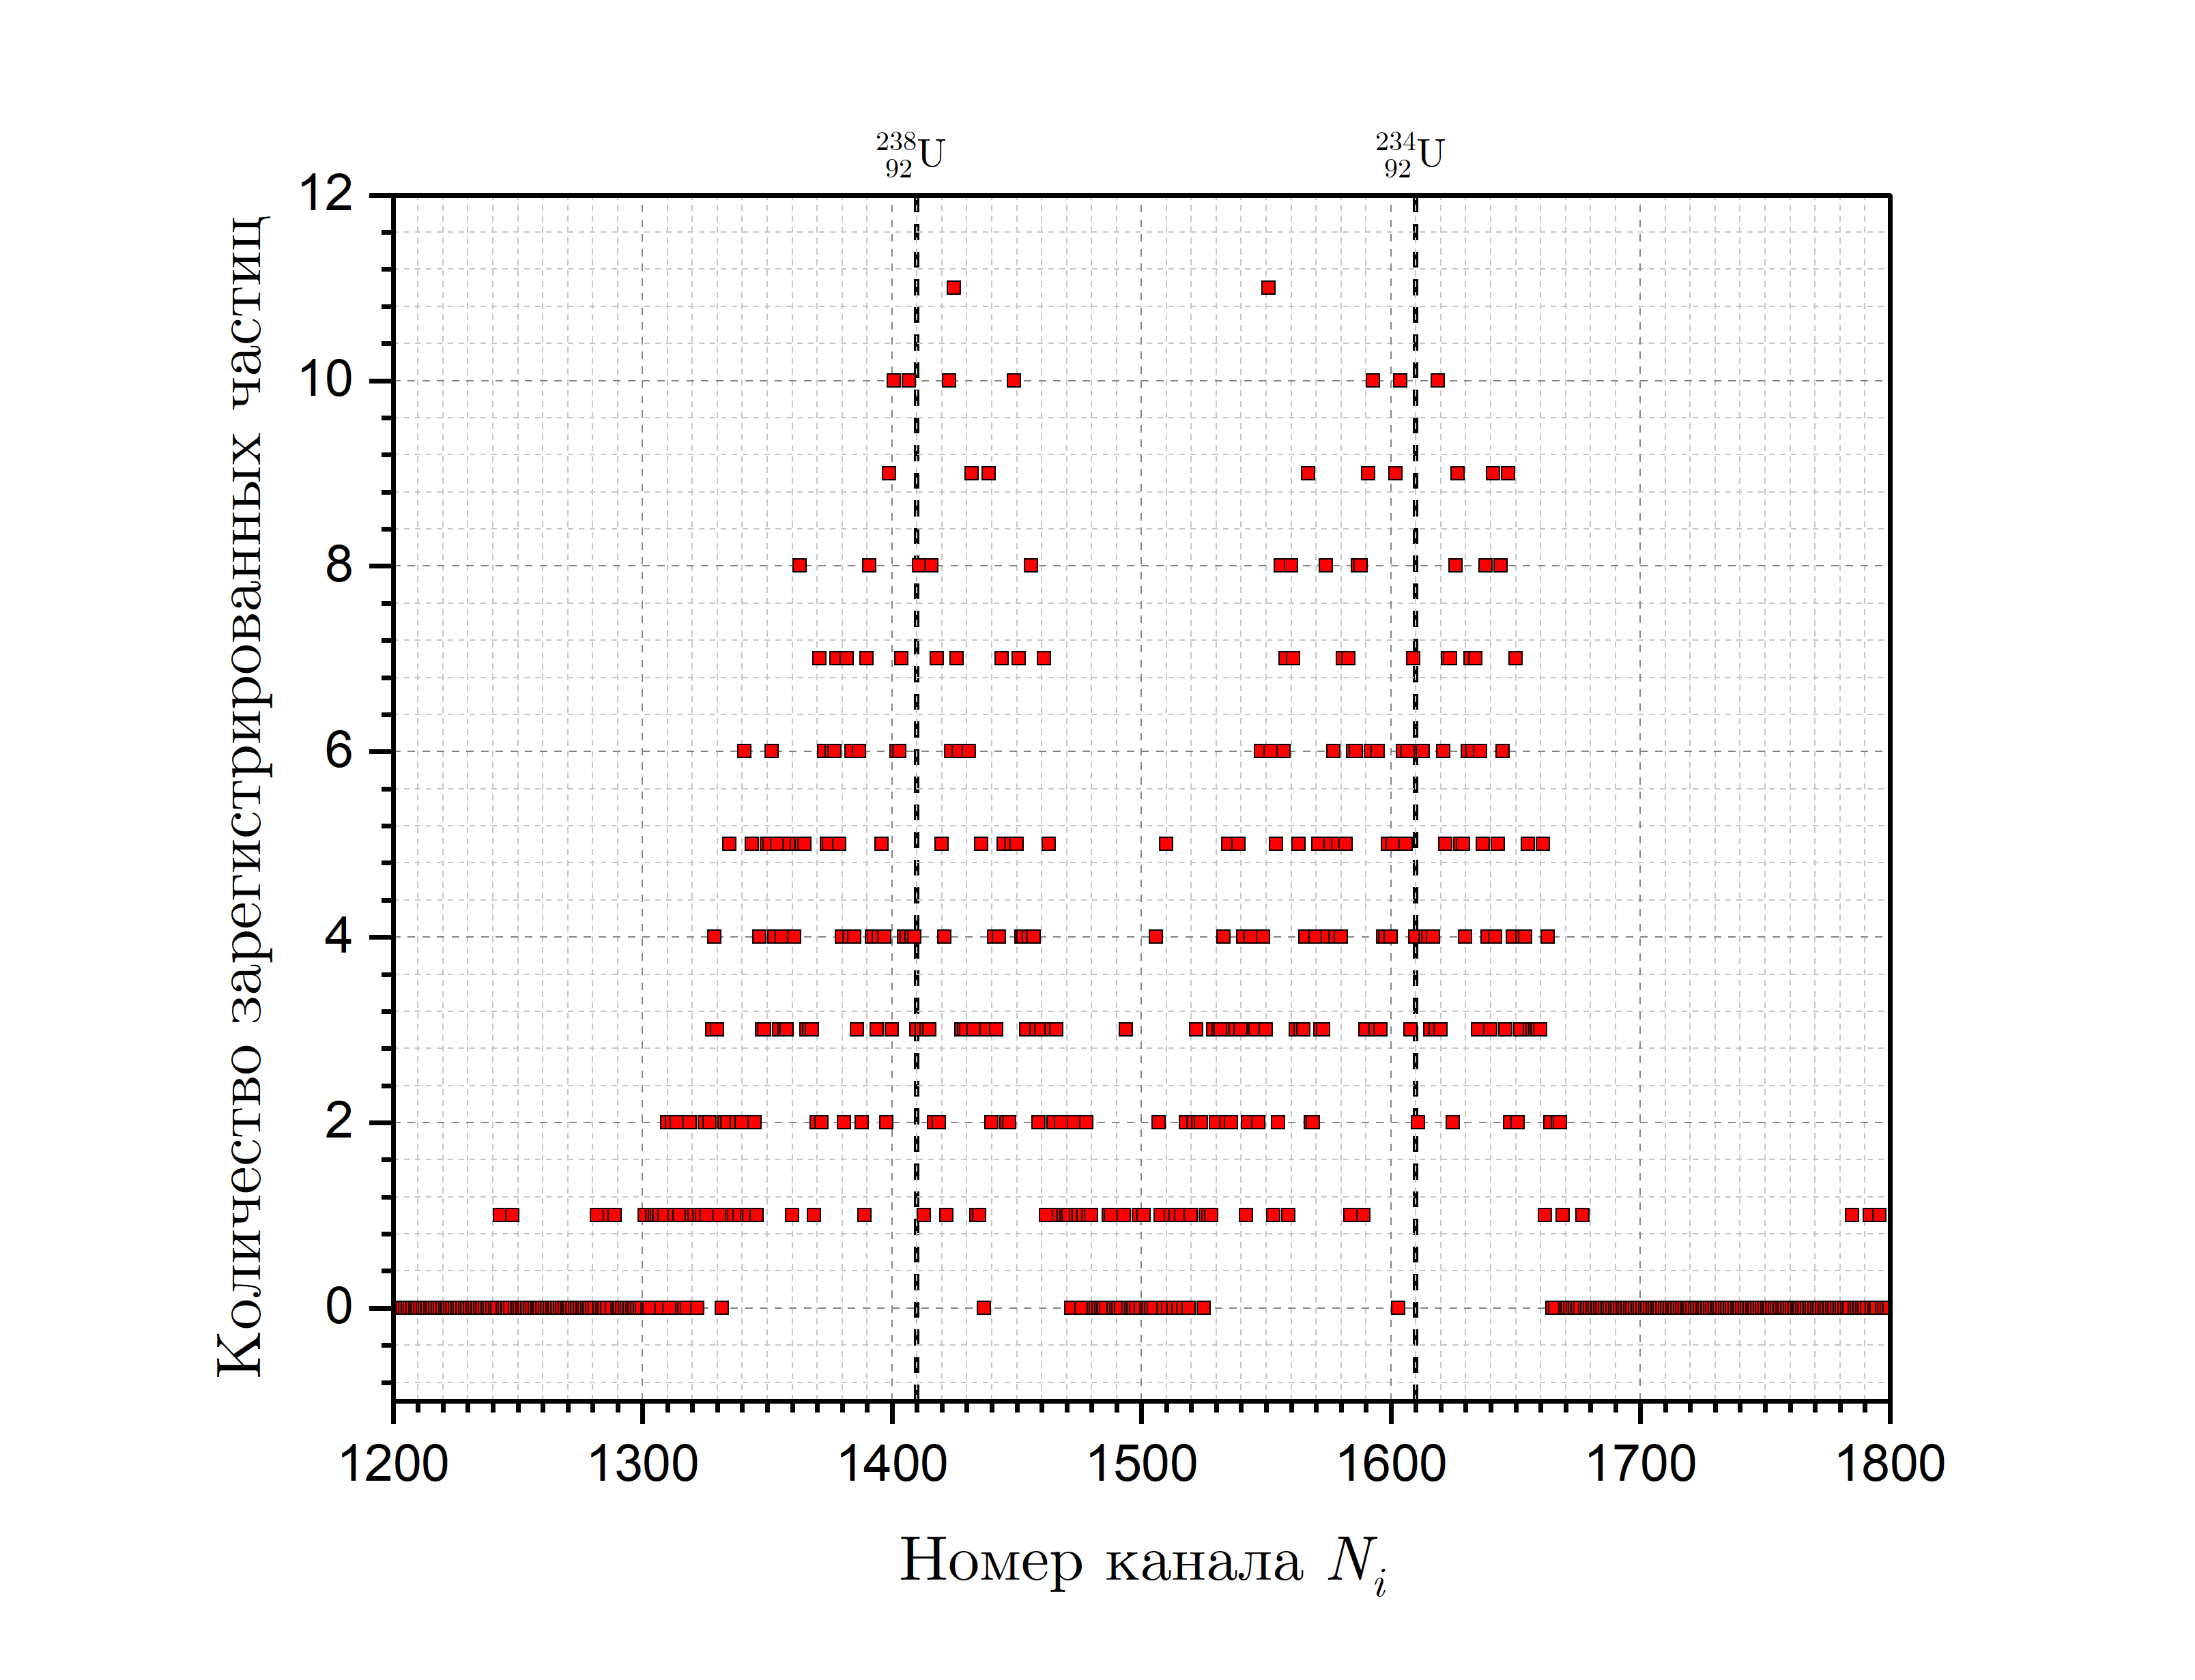
\includegraphics[width = 12 cm]{images/graph_u.png}
        \caption{Спектр $\Ua$.}
        \label{fig:u}
    \end{figure}
    
    \begin{table}[H]
        \centering
        \addtolength{\tabcolsep}{-4pt}
        \footnotesize
        \begin{tabular}{ccccccc}
            \toprule
            $N_i$ & $\Delta N_i$ & $E_i$, МэВ & $\varepsilon_{E_i}, \%$ & $\Delta E_i$, МэВ & $R_i \cdot 10^2$ & $R_{f,i} \cdot 10^2$ \\
            \midrule
            1400 & 87.96 & 4.07 & 0.7 & 0.2614 & 6.43 & 0.094 \\
            1629 & 43.20 & 4.75 & 0.6 & 0.1284 & 2.71 & 0.087 \\
            \bottomrule
        \end{tabular}
        \caption{Энергии пиков $\Ua$.}
        \label{tab:u}
    \end{table}
	
    \subsection{Проверка закона Гейгера-Нэттола}
		
    Зная энергии $\alpha$-распада $\Ra$ и его дочерних ядер, а также периоды их полураспада, можно судить о точности выполнения закона Гейгера-Неттола. С этой целью проведем линеаризацию зависимости:
	
    \begin{figure}[H]
        \centering
        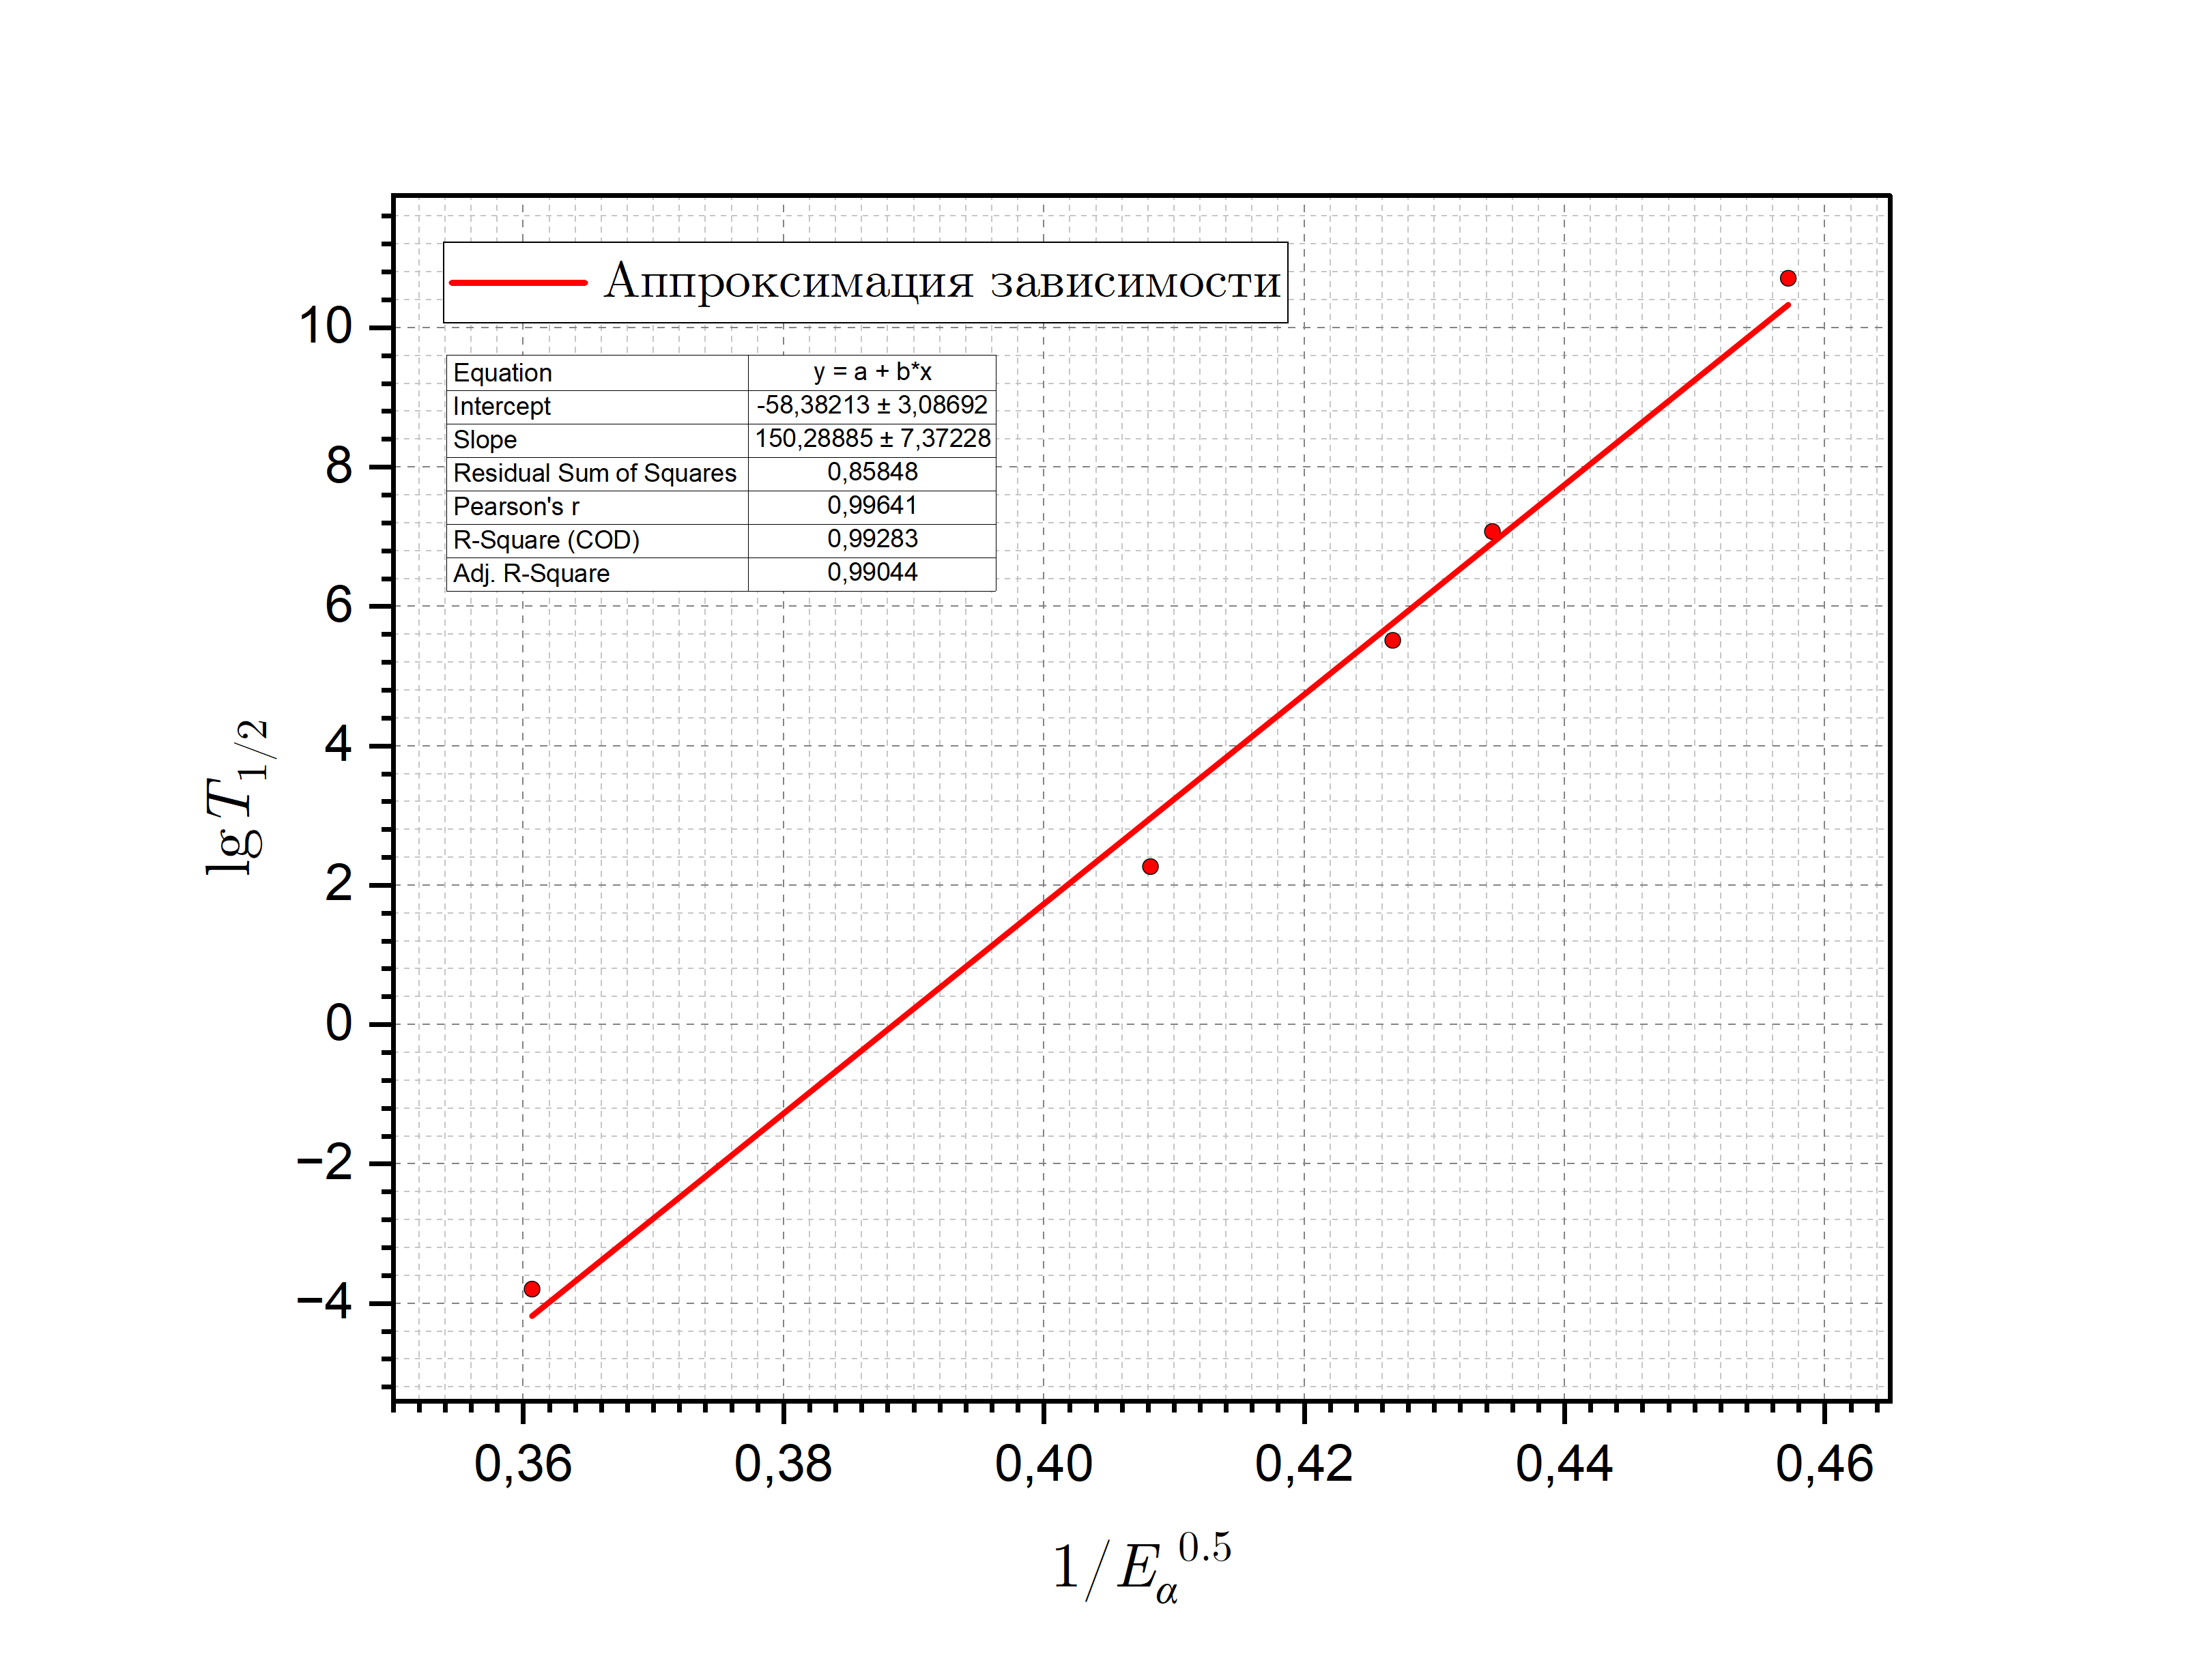
\includegraphics[width = 12 cm]{images/graph_TE.png}
        \caption{График $\log{T_{1/2}} \left( \frac{1}{\sqrt{E_i}}\right)$.}
        \label{fig:te}
    \end{figure}

    \section{Заключение}

    \begin{itemize}
        \item В работе были получены спектры $\alpha$-излучения ядер. Мы экспериментально определили энергетическое разрешение детектора (см. таблицы):
        $$R_i = \frac{\Delta E_i}{E_i},\; \varepsilon_{R_i} \sim 2 \%.$$

        \item Оценка влияния статистической флуктуации числа электрон-дырочных пар $R_{f,i} = \sqrt{\frac{E_{\text{ср}}}{E_i}}, \; \varepsilon_{R_{f,i}} \sim 1.5 \%$, создаваемых падающей частицей, получилась на порядки меньше вычисленных энергетических разрешений $R_i$. Поэтому можно сделать вывод, что основной причиной разброса импульсов по амплитуде является шум электрических цепей.

        \item Был проверен закон Гейгера-Нэттола методом линеаризации зависимости. Коэффициент корреляции слабо отличается от единицы.
    \end{itemize}
    
\end{document}